% The Paley graph P_13: x ~ y iff x - y is a nonzero square mod 13 (squares 1,3,4,9,10,12). srg(13,6,2,3).
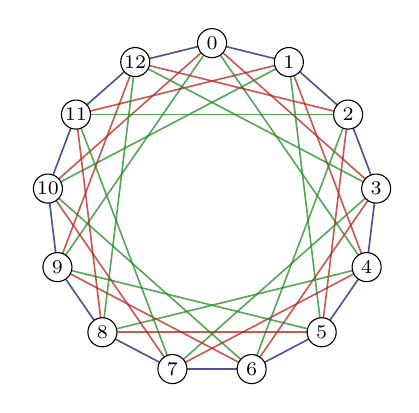
\begin{tikzpicture}[scale=1.05]
\draw[MidnightBlue,semithick,opacity=0.75] (0.000,2.000) -- (0.929,1.771);
\draw[BrickRed,semithick,opacity=0.75] (0.000,2.000) -- (1.985,0.241);
\draw[ForestGreen,semithick,opacity=0.75] (0.000,2.000) -- (1.870,-0.709);
\draw[ForestGreen,semithick,opacity=0.75] (0.000,2.000) -- (-1.870,-0.709);
\draw[BrickRed,semithick,opacity=0.75] (0.000,2.000) -- (-1.985,0.241);
\draw[MidnightBlue,semithick,opacity=0.75] (0.000,2.000) -- (-0.929,1.771);
\draw[MidnightBlue,semithick,opacity=0.75] (0.929,1.771) -- (1.646,1.136);
\draw[BrickRed,semithick,opacity=0.75] (0.929,1.771) -- (1.870,-0.709);
\draw[ForestGreen,semithick,opacity=0.75] (0.929,1.771) -- (1.326,-1.497);
\draw[ForestGreen,semithick,opacity=0.75] (0.929,1.771) -- (-1.985,0.241);
\draw[BrickRed,semithick,opacity=0.75] (0.929,1.771) -- (-1.646,1.136);
\draw[MidnightBlue,semithick,opacity=0.75] (1.646,1.136) -- (1.985,0.241);
\draw[BrickRed,semithick,opacity=0.75] (1.646,1.136) -- (1.326,-1.497);
\draw[ForestGreen,semithick,opacity=0.75] (1.646,1.136) -- (0.479,-1.942);
\draw[ForestGreen,semithick,opacity=0.75] (1.646,1.136) -- (-1.646,1.136);
\draw[BrickRed,semithick,opacity=0.75] (1.646,1.136) -- (-0.929,1.771);
\draw[MidnightBlue,semithick,opacity=0.75] (1.985,0.241) -- (1.870,-0.709);
\draw[BrickRed,semithick,opacity=0.75] (1.985,0.241) -- (0.479,-1.942);
\draw[ForestGreen,semithick,opacity=0.75] (1.985,0.241) -- (-0.479,-1.942);
\draw[ForestGreen,semithick,opacity=0.75] (1.985,0.241) -- (-0.929,1.771);
\draw[MidnightBlue,semithick,opacity=0.75] (1.870,-0.709) -- (1.326,-1.497);
\draw[BrickRed,semithick,opacity=0.75] (1.870,-0.709) -- (-0.479,-1.942);
\draw[ForestGreen,semithick,opacity=0.75] (1.870,-0.709) -- (-1.326,-1.497);
\draw[MidnightBlue,semithick,opacity=0.75] (1.326,-1.497) -- (0.479,-1.942);
\draw[BrickRed,semithick,opacity=0.75] (1.326,-1.497) -- (-1.326,-1.497);
\draw[ForestGreen,semithick,opacity=0.75] (1.326,-1.497) -- (-1.870,-0.709);
\draw[MidnightBlue,semithick,opacity=0.75] (0.479,-1.942) -- (-0.479,-1.942);
\draw[BrickRed,semithick,opacity=0.75] (0.479,-1.942) -- (-1.870,-0.709);
\draw[ForestGreen,semithick,opacity=0.75] (0.479,-1.942) -- (-1.985,0.241);
\draw[MidnightBlue,semithick,opacity=0.75] (-0.479,-1.942) -- (-1.326,-1.497);
\draw[BrickRed,semithick,opacity=0.75] (-0.479,-1.942) -- (-1.985,0.241);
\draw[ForestGreen,semithick,opacity=0.75] (-0.479,-1.942) -- (-1.646,1.136);
\draw[MidnightBlue,semithick,opacity=0.75] (-1.326,-1.497) -- (-1.870,-0.709);
\draw[BrickRed,semithick,opacity=0.75] (-1.326,-1.497) -- (-1.646,1.136);
\draw[ForestGreen,semithick,opacity=0.75] (-1.326,-1.497) -- (-0.929,1.771);
\draw[MidnightBlue,semithick,opacity=0.75] (-1.870,-0.709) -- (-1.985,0.241);
\draw[BrickRed,semithick,opacity=0.75] (-1.870,-0.709) -- (-0.929,1.771);
\draw[MidnightBlue,semithick,opacity=0.75] (-1.985,0.241) -- (-1.646,1.136);
\draw[MidnightBlue,semithick,opacity=0.75] (-1.646,1.136) -- (-0.929,1.771);
\fill[white] (0.000,2.000) circle (5pt); \draw[black] (0.000,2.000) circle (5pt);
\node[font=\scriptsize] at (0.000,2.000) {0};
\fill[white] (0.929,1.771) circle (5pt); \draw[black] (0.929,1.771) circle (5pt);
\node[font=\scriptsize] at (0.929,1.771) {1};
\fill[white] (1.646,1.136) circle (5pt); \draw[black] (1.646,1.136) circle (5pt);
\node[font=\scriptsize] at (1.646,1.136) {2};
\fill[white] (1.985,0.241) circle (5pt); \draw[black] (1.985,0.241) circle (5pt);
\node[font=\scriptsize] at (1.985,0.241) {3};
\fill[white] (1.870,-0.709) circle (5pt); \draw[black] (1.870,-0.709) circle (5pt);
\node[font=\scriptsize] at (1.870,-0.709) {4};
\fill[white] (1.326,-1.497) circle (5pt); \draw[black] (1.326,-1.497) circle (5pt);
\node[font=\scriptsize] at (1.326,-1.497) {5};
\fill[white] (0.479,-1.942) circle (5pt); \draw[black] (0.479,-1.942) circle (5pt);
\node[font=\scriptsize] at (0.479,-1.942) {6};
\fill[white] (-0.479,-1.942) circle (5pt); \draw[black] (-0.479,-1.942) circle (5pt);
\node[font=\scriptsize] at (-0.479,-1.942) {7};
\fill[white] (-1.326,-1.497) circle (5pt); \draw[black] (-1.326,-1.497) circle (5pt);
\node[font=\scriptsize] at (-1.326,-1.497) {8};
\fill[white] (-1.870,-0.709) circle (5pt); \draw[black] (-1.870,-0.709) circle (5pt);
\node[font=\scriptsize] at (-1.870,-0.709) {9};
\fill[white] (-1.985,0.241) circle (5pt); \draw[black] (-1.985,0.241) circle (5pt);
\node[font=\scriptsize] at (-1.985,0.241) {10};
\fill[white] (-1.646,1.136) circle (5pt); \draw[black] (-1.646,1.136) circle (5pt);
\node[font=\scriptsize] at (-1.646,1.136) {11};
\fill[white] (-0.929,1.771) circle (5pt); \draw[black] (-0.929,1.771) circle (5pt);
\node[font=\scriptsize] at (-0.929,1.771) {12};
\end{tikzpicture}
